\documentclass{article}

\usepackage{hyperref}
\usepackage{longtable}
\usepackage{array}
\usepackage{booktabs}
\usepackage{graphicx}

\providecommand{\tightlist}{%
  \setlength{\itemsep}{0pt}\setlength{\parskip}{0pt}}

\begin{document}

\tableofcontents

\section{Introduction}\label{introduction}

The Fluid Corpus Manipulation Toolkit (FluCoMa) enables techno-fluent
musicians to use machine listening and machine learning in their
creative practice within the familiar environments of Max,
SuperCollider, and Pure Data. Housed at the University of Huddersfield's
Center for Research in New Music (CeReNeM) in the United Kingdom, the
project's primary development period was funded by a five-year grant
(2017-2022) from the European Research Council.

While the core of the project produced code packages for all three major
computer music programming environments, FluCoMa's vision and impact are
broader. FluCoMa is also a collection of learning resources, code
examples, commissioned artworks, musicological articles, interviews,
podcasts, a philosophy about interface design for creative coding, a
conversation about the future of computer music, a curriculum of machine
listening and machine learning topics, a community of users around the
world, and more. The materials included here extend this ecosystem to
encompass resources for pedagogues that might be used to teach FluCoMa
in various settings. While some of the ideas and resources presented
below are FluCoMa-specific, many of them are toolkit-agnostic and we
hope that they can be used by anyone looking to teach machine listening
and machine learning for creative music making.

The extent of the FluCoMa ecosystem supports our belief that ``providing
the tools'' is not enough to achieve FluCoMa's mission: \emph{enable
techno-fluent musicians to use machine listening and machine learning in
their creative practices}. To truly enable these artists we also must
provide knowledge and inspiration, all in a way that is learnable for
our main user base: computer musicians. Topics in machine listening,
machine learning, computational thinking, and data science are often not
included in the training of electronic musicians and therefore a primary
objective of FluCoMa is to build bridges of understanding from the
knowledge that comes from computer music training to a degree of fluency
with these topics that enables creative music making.

\section{Design Goals}

The learning materials included in this document have been created
through participatory, iterative, and interactive design. The first
draft of learning materials were developed based on feedback from
\href{https://www.flucoma.org/commissions/}{composers} commissioned to
create music with early versions of the Toolkit. Their feedback on what
was confusing about the tools, resources, examples, etc. led to a second
draft of learning materials which were then used in over thirty
workshops around the world with computer musicians from various
backgrounds. The feedback from these workshop participants further
refined the learning materials and have led to the broad ecosystem of
learning resources now found as part of the FluCoMa Toolkit.

\subsection{Tiered Learning Resources}\label{tiered-learning-resources}

Because different learners will desire different degrees of fluency with
these topics, we have tried to tier the learning resources accordingly.
The most proximal resources (such as environment-native
\hyperref[creative-coding-environment-materials]{help files}) provide a
working understanding of what an algorithm does alongside musical
examples of how it might be used. Additional resources (such as the
\hyperref[web-reference]{internet resources}) provide a deeper
understanding that might satisfy one's curiosity and/or build an
intuition of what is happening ``under the hood,'' both of which can
enable a more informed manipulation of the Toolkit. When appropriate, we
also link to the white paper that describes the algorithm from an
engineering perspective, should the learner wish to pursue that amount
of technical detail.

In some cases, paths for pursuing additional resources are more
extensive and less linear. This is especially true for the more complex
tools in FluCoMa, such as neural networks which have multiple dedicated
web resources with varying degrees of technical information, any one of
which might come after an initial introduction, but when taken all
together encompass the degree of fluency we propose for our learners and
users. Learners who are eager to manipulate the many neural network
hyper-parameters might jump to
\href{https://learn.flucoma.org/learn/mlp-parameters/}{MLP Parameters},
while a user who needs a little more time absorbing how a neural network
works might opt for
\href{https://learn.flucoma.org/learn/mlp-training/}{MLP Training}.
(Also see
\href{https://learn.flucoma.org/reference/mlpregressor/}{MLPRegressor},
\href{https://learn.flucoma.org/reference/mlpclassifier/}{MLPClassifier},
and
\href{https://learn.flucoma.org/learn/training-testing-split/}{Training-Testing
Split}.)

Tiered learning resources allow the learner to pursue knowledge as far
as they deem appropriate to feed their creative practice in a given
moment. Providing the learner what they \emph{need} to know \emph{when}
they \emph{need} to know it enables them to stay focused on a creative
idea and not become overwhelmed by what could be a very large body of
knowledge with a daunting learning curve. This sensitivity to the
relationship between creative pursuits and technical knowledge reflects
earlier findings of FluCoMa outlined as ``Techno-Fluency''
and ``Divergence.'' \cite{green2019interdisciplinary} By offering signposts and links to further
resources, the user knows where to keep learning if necessary in the
moment, or, in the future if they decide to continue exploring.

\subsection{Music-Forward Resources}\label{music-forward-resources}

Because of the specificity of our target learner (a creative coding
musician), we have always tried to keep our learning materials and
examples musically oriented (as can be seen below). We aim to have the
help files and example code make sound in a creative way. When possible,
we offer pedagogical examples and thought experiments that will feel
familiar and relevant to our learner such as
\href{https://learn.flucoma.org/reference/noveltyfeature/}{instrument
samples},
\href{https://learn.flucoma.org/reference/bufstats/\#a-musical-example}{drum
hits},
\href{https://learn.flucoma.org/reference/bufstats/\#order-statistics}{MIDI
notes},
\href{https://learn.flucoma.org/learn/regression-neural-network/}{synthesizer
settings},
\href{https://learn.flucoma.org/learn/why-scale/\#plotting-sound-slices-where-1-hz--1-db}{measures
of frequency and loudness}, etc. We hope this strategy will not only
explain a tool and its interface, but also provide some
copy-and-paste code to get started quickly, and generally get the
musical creative juices flowing while a user is engaging in the learning
process.

\section{Ecosystem of Learning Materials}\label{ecosystem-of-learning-materials}

\subsection{Creative Coding Environment Materials}\label{creative-coding-environment-materials}

Each creative coding environment (CCE) supported by FluCoMa (Max,
SuperCollider, and Pure Data) has a native system for offering reference
materials. In Max and Pure Data a ``help file'' provides annotated
examples, while a ``reference'' offers additional description and detail
about parameters. In SuperCollider all of this information is contained
in one ``help file'' document. Despite this difference in interface, we
have strived to keep the CCE-based FluCoMa materials similar across all
three environments. This is enabled, in part, by the
\href{https://github.com/flucoma/flucoma-docs}{shared documents used to
render the reference materials} for all three CCEs.

The FluCoMa materials provided natively in the CCE are often the
learner's first engagement with our supporting materials. Therefore, the
information provided is intended to provide the learner/user a working
understanding of what an object does, how it might be used musically
through a sound-making example, and if appropriate, how it interfaces
with other FluCoMa objects. This information will hopefully provide a
learner some motivation for exploring an object and the amount of
knowledge necessary to do so. Each resource in the CCE contains a link
to the corresponding \hyperref[web-reference]{web-reference} if the
learner wishes to pursue a deeper understanding of the object.

The example code provided has been created to be as similar as possible
across the three CCEs while keeping idiomatic to each environment. One
goal of this is to enable cross-environment communication and knowledge
sharing. Users in different CCEs are able to discuss the technical and
musical facets of a shared FluCoMa example. It is also possible that
this allows referencing help files and example code to a classroom
containing a diversity of coding environment users. Lastly, this keeps
all three CCEs on an equal status, preventing any potential inference of
CCE preference within the FluCoMa Toolkit.

\subsection{Web Reference}\label{web-reference}

Every object in FluCoMa (except
\hyperref[cce-specific-objects]{CCE-specific objects}) has a web
reference found at \href{https://learn.flucoma.org}{learn.flucoma.org}.
Because the reference materials that appear natively in the CCEs link to the web,
the web references are considered to be a secondary resource. The goal
of the web references is to offer more detailed descriptions of how an
algorithm is working ``under the hood''. This may be useful for
satisfying curious learners and/or building a better intuition for
musical uses of an object. In either case, it could lead to a more
informed, and therefore potentially more advanced, use of the object.

Many of the web references have interactive explanations that allow a
learner to ``use'' the algorithm in the browser. Not only can these be
used by individual learners, we have also found that these are very
useful for explanations in the course of teaching. For example, when
creating a KDTree for the first time during a code-along class, using
the \href{https://learn.flucoma.org/reference/kdtree/}{interactive page}
helps give learners a visual sense of what is happening (especially if
the KDTree is about to be used with the plotter). The
\href{https://learn.flucoma.org/reference/mfcc/}{MFCC reference} has an
\href{https://learn.flucoma.org/reference/mfcc/explain/}{interactive
explanation} that invites a learner (or a teacher during demonstration)
to step through a series of interactions that build intuition about
MFCCs.

We imagine the web references to be used as solo-learning resources, in
parallel with class assignments, as teaching demonstrations, and/or as
useful reminders.

\subsection{Learn Articles}\label{learn-articles}

FluCoMa's learning website
(\href{https://learn.flucoma.org}{learn.flucoma.org}) also contains many
articles about topics that may not fit in a single web reference page.
These articles may arise as a tertiary step in a learners path and are
likely to be encountered after the CCE materials and web reference.

There are a few varieties of articles found in this category:

\begin{itemize}
\tightlist
\item
  explainers specific to a single FluCoMa object that offer a depth of
  knowledge about the internal algorithms that would be outside the
  scope of a web reference page, such as
  \href{https://learn.flucoma.org/learn/bufnmf/}{Audio Decomposition
  using BufNMF}.
\item
  knowledge about data science that is useful for using many of the
  FluCoMa objects, such as
  \href{https://learn.flucoma.org/learn/distribution/}{Distribution and
  Histograms} and \href{https://learn.flucoma.org/learn/why-scale/}{Why
  Scale? Distance as Similarity}
\item
  common workflows using the toolkit, such as
  \href{https://learn.flucoma.org/learn/batch-processing/}{Batch
  Processing with FluCoMa}
\end{itemize}

These articles are not necessarily designed to be consumed in series as
part of a sequence of learning (although some could be used this way).
Instead, each article is made to be approached by a learner (or guided
by a teacher) at a particular point in the learning process and
revisited as necessary. The idea for many of these articles arose in
direct response to questions asked by workshop participants and
therefore are designed to answer or provide context to common questions
asked by learners. When designing a curriculum or syllabus, many of these
articles would support student learning for different topics in a
course.

\subsection{Explore Articles}\label{explore-articles}

In addition to the web reference and learn articles, the website has
many \href{https://learn.flucoma.org/explore/}{additional materials}
surrounding artistic uses of the toolkit. These include example
artworks, interviews with creative coders, and musicological articles
that offer in-depth analysis and example patches of music made with
FluCoMa. All of these can be used as context, examples, and inspiration
for learners. These can also be used as entry points, as many learners
will find the work produced using FluCoMa or the musical ideas expressed
in these articles inspiring and motivating.

\subsection{Discourse}\label{discourse}

The international community of FluCoMa users primarily communicates
through the \href{https://discourse.flucoma.org/}{Discourse} online
discussion forum. Any learner (or user) of FluCoMa should be a member of
the Discourse as it is an excellent place to converse with like-minded
artists. Learners may find the search functionality very useful to see
if others have already asked and answered a question they have. The
community is very positive and supportive, so it is a safe place to ask
all kinds of questions. In addition to the thread for
, \href{https://discourse.flucoma.org/c/getting-started-and-wayfinding}{\emph{Getting Started and Wayfinding}}, 
\href{https://discourse.flucoma.org/c/usage-questions}{\emph{Usage Questions}}, there are also threads for
\href{https://discourse.flucoma.org/c/code-sharing}{\emph{Code Sharing}},
\href{https://discourse.flucoma.org/c/learning-resources}{\emph{Learning Resources}}, and
\href{https://discourse.flucoma.org/c/interesting-links}{\emph{Interesting Links}} 
making it another place for learners to browse for examples,
inspiration, and knowledge.

\subsection{Inter-connectivity of
Resources}\label{inter-connectivity-of-resources}

As described above, the FluCoMa learning resources are generally tiered
to offer learners the degree of detail needed at a given moment to
pursue a creative idea. One way in which our tiered approach is executed
is cross referencing the different learning resources. The help files in
each creative coding environment (CCE) link to their respective web
reference, from which a learner can be pointed to many more resources.
The web reference, learn articles, and explore articles all cross-link
with each other so that a learner reading a web reference might discover
an Explore Article about a musician's use of an object, and from there
discover a Learn Article to help them pursue the creative use they just
learned about, etc. Different learners will need different degrees of
technical specificity, inspiration, and modes of engagement at different
times. We hope that setting someone ``loose'' on the website will enable
them to find uses of FluCoMa that are meaningful to them as well as the
knowledge needed to support them.

\begin{figure}[ht]
\centering
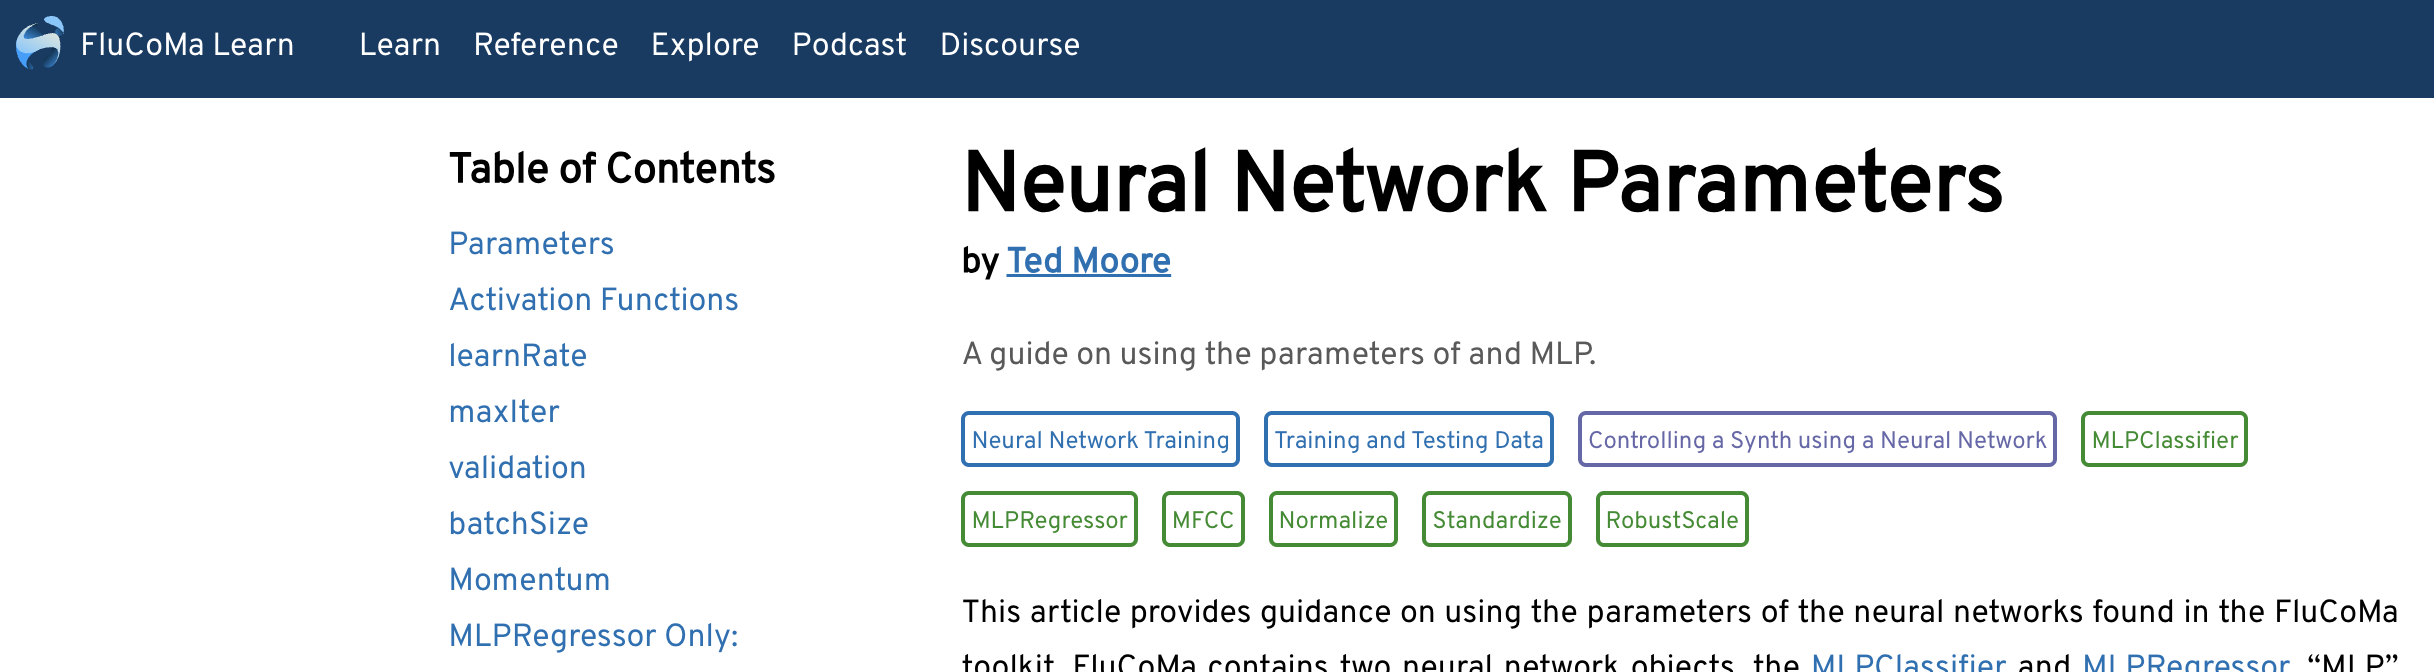
\includegraphics[width=0.9\textwidth]{./figures/interconnected-resources.png}
\caption{Screenshot from "Neural Network Parameters" page showing links to other related pages as colored boxes.}
\label{fig:interconnected-resources}
\end{figure}

\section{Example Lesson Plan: MLPRegressor}\label{example-lesson-plan}

After teaching numerous workshops we have identified a few class plans
that work well to get new learners excited and making sound while laying
a foundation of facility with FluCoMa to support further activities
and/or self-guided learning. The lesson plan summarized here introducing neural networks with the MLPRegressor is often as a first instruction to FluCoMa.

\textbf{Watch a Video Tutorial of this Lesson Plan}

\begin{itemize}
\tightlist
\item
  \href{https://www.youtube.com/watch?v=XfNZzQPdPG0}{MLPRegressor in
  Max}
\item
  \href{https://www.youtube.com/watch?v=mxmMBvi3Cb0}{MLPRegressor in
  SuperCollider}
\end{itemize}

The first activity that we often engage learners with is building a
neural network that performs regression to control a synthesizer with ten control parameters from a space of only two parameters. This
gets learners making sound quickly and uses part of the toolkit that is
often quite exciting for newcomers to machine learning (neural
networks). This activity takes any where from 40-90 minutes depending on
the class of learners. Here is a brief outline of the lesson plan:

\begin{enumerate}
\def\labelenumi{\arabic{enumi}.}
\tightlist
\item
  Share a
  \href{https://f003.backblazeb2.com/file/learnassets/examples/teaching-material/regressor-example.pdf}{real
  world example} (including watching a
  \href{https://vimeo.com/565771489}{performance excerpt}) of why
  someone might want to use a system like this.
\item
  Using a
  \href{https://f003.backblazeb2.com/file/learnassets/examples/teaching-material/regressor-process.pdf}{slides
  presentation} step through how we will be collecting training data and
  training the neural network, including some intuition about how the
  training process works.
\item
  Open up the CCE of choice and demonstrate a completed version
  (\href{https://learn.flucoma.org/examples/regressor-video-demo.maxpat}{Max},
  \href{https://learn.flucoma.org/examples/regressor-video-complete-server.scd}{SuperCollider})
  of the instrument we're about to code.
\item
  Code the instrument together, as a code-along, starting from a
  ``starter patch''
  (\href{https://learn.flucoma.org/examples/regressor-video-starter.maxpat}{Max},
  \href{https://learn.flucoma.org/examples/regressor-video-starter.scd}{SuperCollider})
  that has a few key items already in place:

  \begin{itemize}
  \tightlist
  \item
    a synthesizer to control
  \item
    a 2D control space to use as input to the neural network
  \item
    a MLPRegressor object with many arguments already specified
  \end{itemize}
\item
  Let the learners play with the instrument (and augment it in their own
  way).
\end{enumerate}

The starter patch is important here so that we don't spend too
much time doing CCE-specific boiler plate code but instead get right
into using FluCoMa. It also ensures that learners have a synthesizer to
make sound with right away when the code-along is complete. Because
there are many arguments to the MLPRegressor object and each of them can
require a fair amount of explanation to use well--and in coordination
with each other--we've chosen to provide the arguments to the
MLPRegressor programmed into the starter patch. During the lesson we
tell the learners that these arguments can be explored further in a
future lesson and/or in the
\href{https://learn.flucoma.org/learn/mlp-parameters/}{learn article}.

The extensions of this activity are to:

\begin{enumerate}
\def\labelenumi{\arabic{enumi}.}
\tightlist
\item
  Practice training the neural network.

  \begin{itemize}
  \tightlist
  \item
    clearing the neural network and retraining
  \item
    training the neural network to a different degree to see if it is more (or less, or differently) musically
    expressive
  \item
    delete the input data and choose new data points to pair with the
    synthesis parameters
  \item
    delete all the data and create a whole new training
  \end{itemize}
\item
  Attach a different sound-making algorithm to the output of the neural
  network

  \begin{itemize}
  \tightlist
  \item
    granular synthesis / sample playback
  \item
    frequency modulation
  \item
    a VST plugin
  \item
    we have often encouraged learners to bring a sound-making algorithm
    of their design to the workshop to connect as a next step to this
    activity
  \end{itemize}
\item
  Attach a different type of controller to the input of the neural
  network. This might be something like:

  \begin{itemize}
  \tightlist
  \item
    multiple parameters on TouchOSC
  \item
    MIDI controller
  \item
    leap motion
  \item
    wearable device
  \item
    pixel information from a camera (perhaps using Jitter in Max)
  \end{itemize}
\end{enumerate}

Not only does this activity quickly provide learners with a machine
learning instrument that is very extensible, it also introduces some of
the key elements of FluCoMa:

\begin{enumerate}
\def\labelenumi{\arabic{enumi}.}
\tightlist
\item
  DataSets
\item
  Buffer interfacing

  \begin{itemize}
  \tightlist
  \item
    \texttt{fluid.buf2list\textasciitilde{}} and
    \texttt{fluid.list2buf\textasciitilde{}} for Max
  \item
    \texttt{FluidBufToKr} and \texttt{FluidKrToBuf} for SuperCollider
  \item
    \texttt{array\ set} and \texttt{array\ get} in Pure Data
  \end{itemize}
\item
  Using small, personalized, artist-created DataSets
\item
  Aesthetic evaluation of results
\item
  Iterative trial-and-error workflows with machine learning algorithms
\end{enumerate}

\subsection{Classifier Extension}\label{classifier-extension}

After completing the MLPRegressor activity, one common extension is to
do an activity training the MLPClassifier to distinguish between two timbres. Depending on the group of
learners and how much time is available, sometimes this would only
include opening up the classifier demonstration file
(\href{https://learn.flucoma.org/examples/classification-video-demo.maxpat}{Max},
\href{https://learn.flucoma.org/examples/classification-video-demo.scd}{SuperCollider})
and doing a quick training and testing, along the way relating it to
what was just done with the MLPRegressor activity. If time allowed and
there is interest we performed a more involved activity similar to the
MLPRegressor: demoing the code and then building it together.

\textbf{Watch a Video Tutorial of this Lesson Plan}

\begin{itemize}
\tightlist
\item
  \href{https://www.youtube.com/watch?v=Y1cHmtbQPSk}{MLPClassifier in
  SuperCollider}
\item
  \href{https://www.youtube.com/watch?v=cjk9oHw7PQg}{MLPClassifier in
  Max}
\end{itemize}

\begin{enumerate}
\def\labelenumi{\arabic{enumi}.}
\tightlist
\item
  Share a
  \href{https://f003.backblazeb2.com/file/learnassets/examples/teaching-material/classifier-example.pdf}{real
  world example} (including watching a performance excerpt, this one has
  a \href{https://youtu.be/8QtvjMUGGB8}{before and after}) of why
  someone might want to use a system like this.
\item
  Using a
  \href{https://f003.backblazeb2.com/file/learnassets/examples/teaching-material/classifier-process.pdf}{slides
  presentation} step through how we will be collecting training data and
  training the neural network, including some intuition about how the
  training process works.
\item
  Open up the CCE of choice and demonstrate a completed version
  (\href{https://learn.flucoma.org/examples/classification-video-demo.maxpat}{Max},
  \href{https://learn.flucoma.org/examples/classification-video-demo.scd}{SuperCollider})
  of what we're about to code.
\item
  Code-along, starting from a ``starter patch''
  (\href{https://learn.flucoma.org/examples/classification-video-starter.maxpat}{Max},
  \href{https://learn.flucoma.org/examples/classification-video-starter.scd}{SuperCollider})
  that has a few key items already in place:

  \begin{itemize}
  \tightlist
  \item
    the sound files containing timbres that will be used as training and testing data
  \item
    a MLPClassifier object with many arguments already specified (for the same reason described above)
  \end{itemize}
\item
  Let the learners explore classifying some of their own sounds
\end{enumerate}

\section{Common Learning Challenges \& Strategies}\label{common-learning-challenges-strategies}

Over the course of teaching many workshops, we observed some common
challenges for FluCoMa learners. Below are a few of the challenges we
found and some strategies for approaching them pedagogically.

\subsection{New Ways of Using Buffers}\label{new-ways-of-using-buffers}

FluCoMa uses buffers to store all kinds of data, not just audio. This
may be new for learners who are used to using buffers \emph{only} for
holding audio, and may even associate the two as a single concept
(``buffer == audio''). This becomes increasingly complicated when we
begin to manipulate the data in buffers as arrays and matrices.

\subsubsection{Initial Encounter}

The first moment at which a learner is asked to view a buffer in a new
way is often when we allocate a buffer to hold a data point. If the data
point has just 2 dimensions (such as with the
\hyperref[example-lesson-plan]{MLPRegressor activity}), we will allocate the
buffer with only 2 frames (in Max: \texttt{@samps\ 2}; in SuperCollider:
\texttt{Buffer.alloc(s,2)}). At this point we try to offer something
like the following:

\begin{quote}
\emph{``The way we most often use buffers in {[}this CCE{]} is to hold
audio samples which very commonly have 44,100 samples per second, so our
buffers could have many tens or hundreds of thousands of values in them.
Because I know this buffer is only going to need to hold two values,
I'll allocate it to have just two samples.''}
\end{quote}

\subsubsection{Holding Analyses}

Once we start writing audio analyses into buffers (with the
\texttt{feature} argument), learners often have a hard time keep track
of the structure of the buffers (What do the channels represent? How
many are there? What do the frames represent? How many are there?). We
found that offering CCE-agnostic
\href{https://f003.backblazeb2.com/file/learnassets/examples/teaching-material/buffer-charts.pdf}{charts}
of the ``shape'' of the buffer is very helpful for giving learners a
mental model to hold in their mind.

\begin{figure}[ht]
\centering
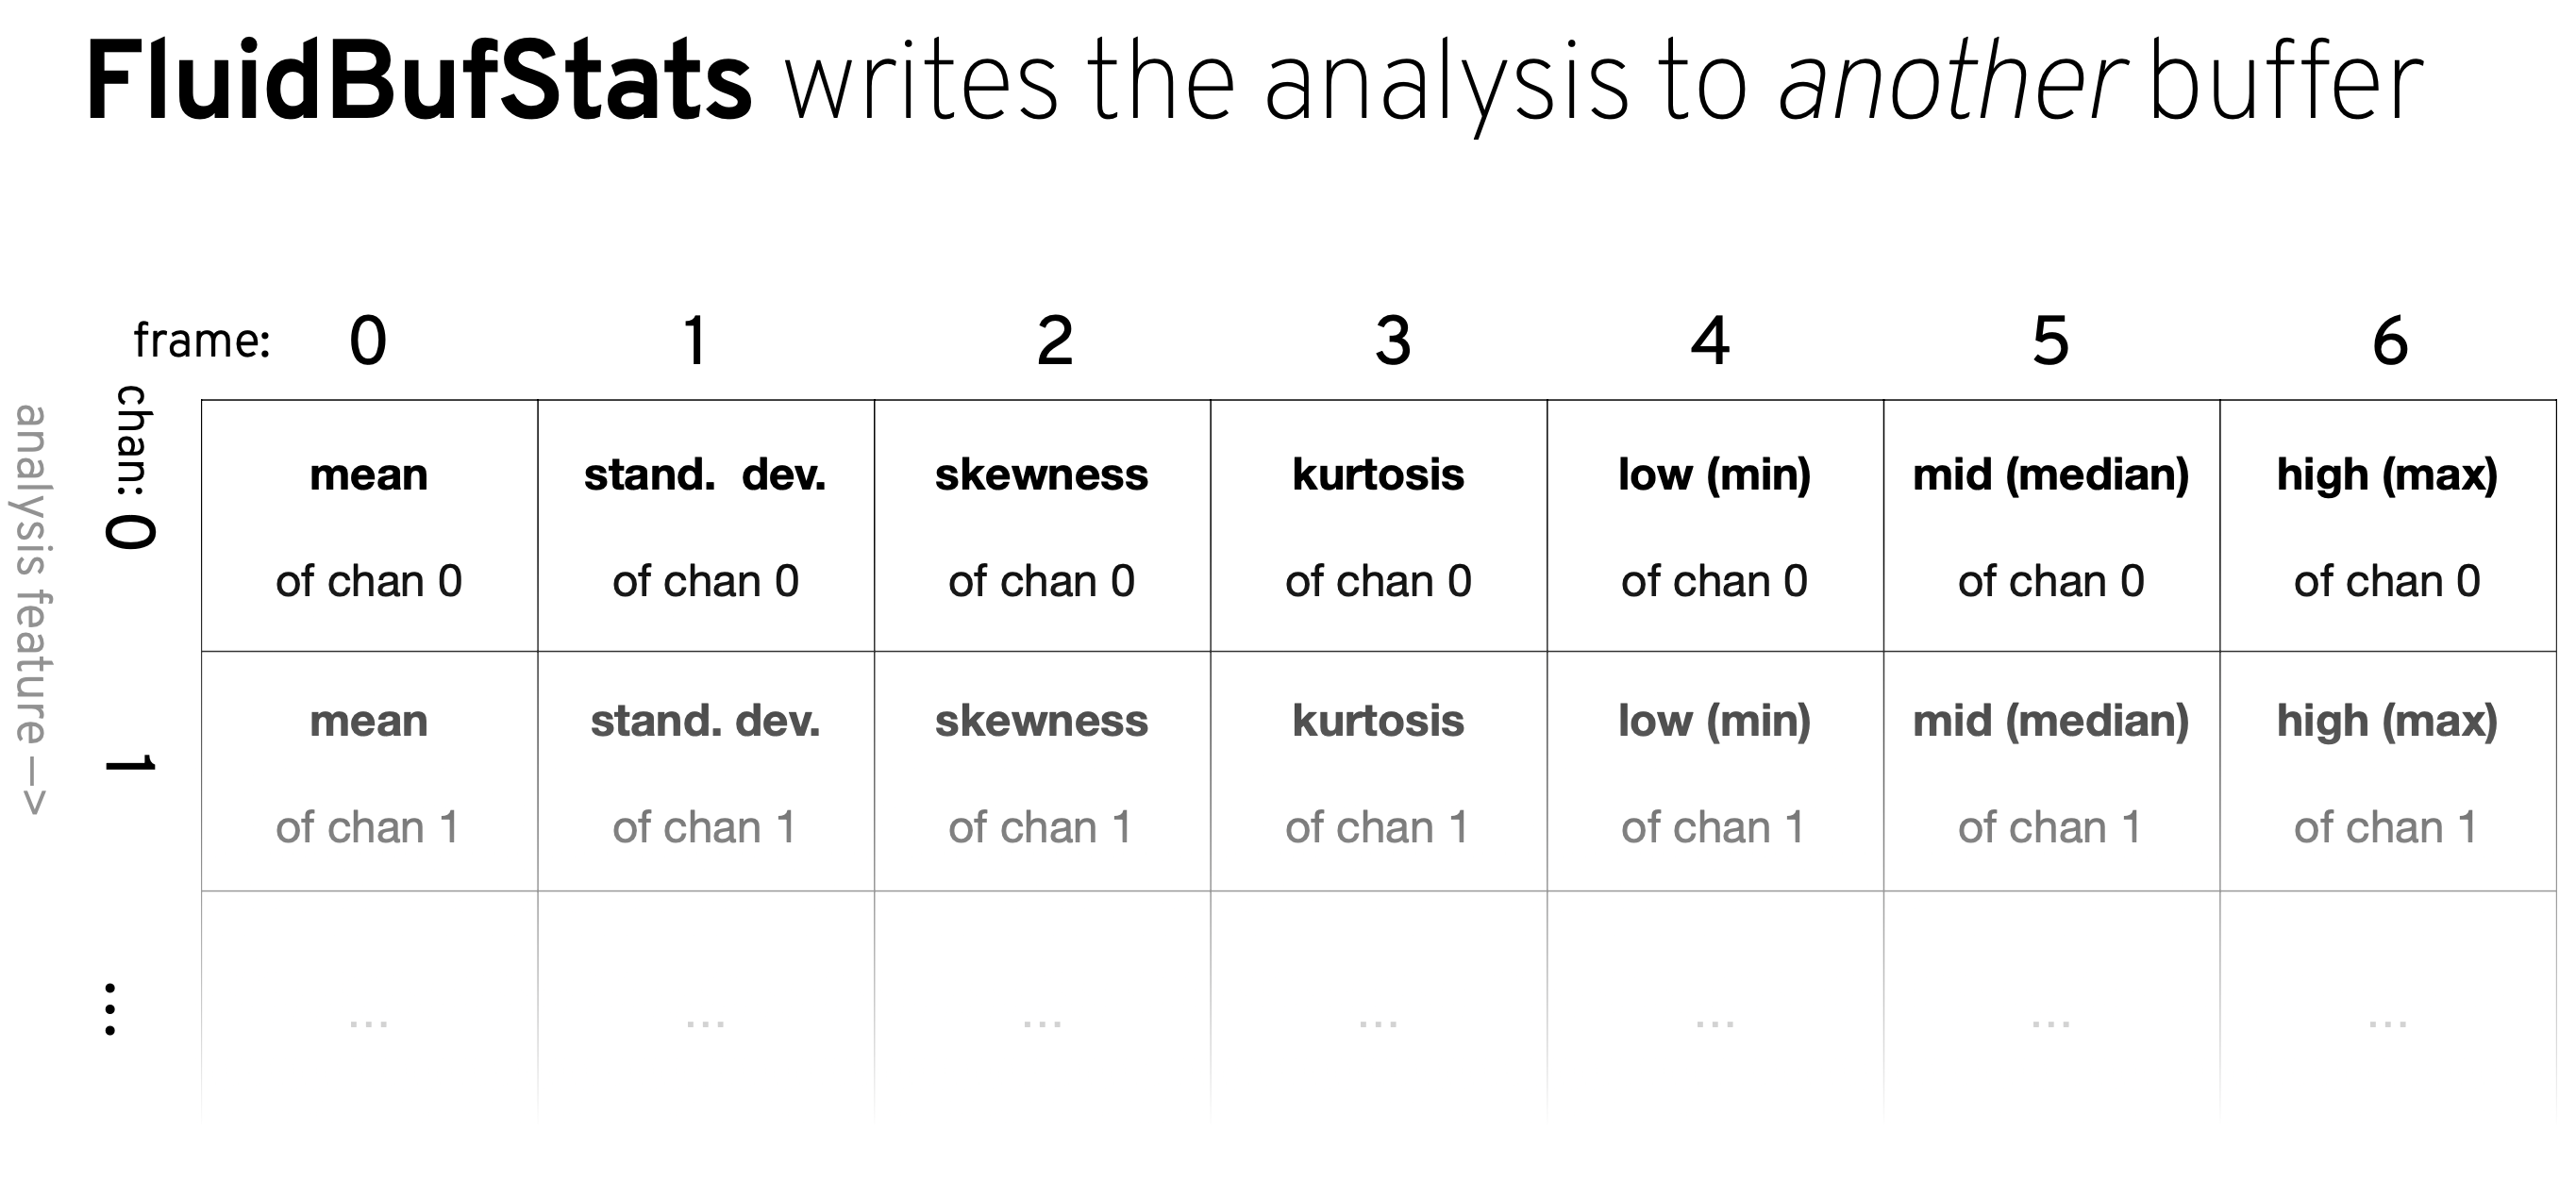
\includegraphics[width=0.9\textwidth]{./figures/bufstats-chart.png}
\caption{Chart demonstrating what the channels and frames of a particular buffer represent.}
\label{fig:bufstats-chart}
\end{figure}

It's also useful to point out that for buffers that hold audio analyses,
the frames (or what we sometimes refer to as the ``\texttt{x} axis'' in
reference to the charts above) is still a time series, just like audio
is, but now it's not a time series of voltages (as in audio), it's a
time series of descriptors (such as spectral centroid).

Because each frame represents an FFT frame from the STFT analysis, the
sample rate would not be a usual 44,100 samples per second, but a much
lower rate of frames per second (FFT frames per second). For example, if
an audio buffer with a sample rate is 44,100 Hz is analyzed with a
\texttt{hopSize} of 512 samples, the \texttt{features} buffer that the
analyses get written into will have a sample rate of 86.1328125 frames
per second (44100 / 512). In SuperCollider and Max, FluCoMa buffer
processors (such as the audio descriptor analyzers) set the \emph{sample
rate} of these buffers appropriately (Pure Data arrays don't hold
metadata). If the values in that buffer are read back at that rate, they
will correspond in time (be synchronized with) to the audio on which the
analysis was based. Point this out to learners helps them remember an conceptualize the relationship between the source audio being analyzed, the STFT process, and the resulting time series of descriptor values.

\subsubsection{Manipulating \& Copying Data}

Often it is necessary to manipulate the data in a buffer, such as pick
out values from certain channels and/or frames and copy them to another
buffer. In order to provide some ``test and check'' interactivity to build
fluency with these operations, the appropriate web references have
interactive GUIs for practicing:

\begin{itemize}
\tightlist
\item
  \href{https://learn.flucoma.org/reference/bufselect/}{BufSelect}
\item
  \href{https://learn.flucoma.org/reference/bufselectevery/}{BufSelectEvery}
\item
  \href{https://learn.flucoma.org/reference/bufflatten/}{BufFlatten}
\item
  \href{https://learn.flucoma.org/reference/bufcompose/}{BufCompose}
\item
  \href{https://learn.flucoma.org/reference/bufscale/}{BufScale}
\end{itemize}

\subsubsection{Why Buffers}

It also may be of interest for learners to hear the explanation of
\emph{why} buffers are used in this way. FluCoMa uses buffers in this
way for a few reasons:

\begin{itemize}
\tightlist
\item
  The notion of ``buffer'' is shared across all three CCEs that FluCoMa
  supports. This allows for shared syntax and usage of objects across
  all three environments.
\item
  In all three CCEs, buffers are accessed at the lower levels of code
  allowing for:

  \begin{itemize}
  \tightlist
  \item
    Faster processing by interfacing directly with the C++ code.
  \item
    Simpler implementation of functions across all three CCEs because
    all three environments share the same C++ code base for all of the
    audio analysis, buffer processing, and algorithms.
  \end{itemize}
\item
  Having data in buffers allows for it to be more flexibly accessed and
  used in other parts of the CCE. For example because the MLPRegressor
  writes predictions into a buffer, it's possible to be predicting
  wavetable shapes directly into a
  buffer that is simultaneously being read out of, all on the scsynth server.
\end{itemize}

\subsection{Stateful Objects}\label{stateful-objects}

Many of the FluCoMa data objects hold some state. For example after
calling \texttt{fit} (or \texttt{fitTransform}) on a Normalize object,
it holds the minimum and maximum value of each dimension in the fitted
DataSet so that it can scale future \texttt{transform} calls
appropriately. MLP objects hold the state of the MLP internal parameters
(the state of the trained model). This interface design is based on many
of the data processing objects in the Python
\href{https://scikit-learn.org/stable/}{sci-kit learn} package. We found
that some FluCoMa learners find it challenging to conceptualize or
remember that certain objects are holding a state that they will need to
call upon later. One feature that may help with conceptualizing objects
in this way is the option to \emph{name} objects in Max and Pure Data
(SuperCollider natively uses variable names to identify objects).

Named objects may help learners remember that certain objects hold state
because they have a sense of it being a non-generic, task-specific
object, such as a Normalize object called \texttt{norm-pre-pca}. This gives
it a special sense of purpose and an indicator of what state it holds
and where in data processing one would call upon that state.

\subsection{Fourier Transform \& STFT}\label{fourier-transform-stft}

As with many audio tasks, the STFT is central to much of how a learner
interacts with FluComa. Many times learners can do exciting things,
learn a lot about the toolkit, and make great music without reflecting
on the FFT processes happening ``under the hood.'' We have found
however, that for many of the algorithms in FluCoMa (such as
\href{https://learn.flucoma.org/reference/audiotransport/}{AudioTransport},
\href{https://learn.flucoma.org/reference/sines/}{Sines}, and many
more), adjusting STFT settings (\texttt{windowSize}, \texttt{hopSize},
and \texttt{fftSize}) has an important aesthetic impact on the results,
and therefore we suggest that it is important to understand what impact
these parameters have.

There exists a
\href{https://learn.flucoma.org/learn/fourier-transform/#related-resources}{wealth
of resources} on the internet for learners to build fluency with the
Fourier Transform, so we didn't feel the need to recreate many of these
learning tools. We have however, curated a small set of musician-oriented ideas that will be important for FluCoMa learners to consider as they are approaching the
toolkit, which exist on these two pages:

\begin{itemize}
\tightlist
\item
  \href{https://learn.flucoma.org/learn/fourier-transform/}{Fourier
  Transform}
\item
  \href{https://learn.flucoma.org/reference/bufstft/}{BufSTFT}
\end{itemize}

\subsection{Advanced Neural Networks}\label{advanced-neural-networks}

Learners often follow up the \hyperref[example-lesson-plan]{MLPregressor Lesson Plan} with questions about the hyper-parameters (which FluCoMa calls
parameters or arguments) of the MLP. In shorter workshops (two days or
fewer) we have felt that it's not enough time to delve into this with
enough depth to make it well understood and \emph{useable} for the
participants, so we've directed them towards our
\href{https://learn.flucoma.org/learn/mlp-parameters/}{web resources} on
the topic. In longer workshops (three days or more) we have taken time
later in the week (day three or four) after the introductory activity to
unpack many more ideas and strategies about the MLP objects.

\subsubsection{Web Resources}

\begin{itemize}
\tightlist
\item
  \href{https://learn.flucoma.org/learn/mlp-training/}{Neural Network
  Training} is an overview of how neural networks learn. It is intended
  for those who would benefit from gaining a little more intuition about
  what is going on ``under the hood'' or for learners that have a little
  more curiosity they want to satisfy. Much of what this article expresses is included in the introductory activity.
\item
  \href{https://learn.flucoma.org/learn/mlp-parameters/}{Neural Network
  Parameters} goes through each parameter in the MLP objects and gives a
  more thorough description of what it controls, why one might adjust
  it, and what a generally reasonable starting place is. This is often
  where we direct learners who ask about these parameters when we don't
  have time to unpack them during a workshop.
\item
  \href{https://learn.flucoma.org/learn/training-testing-split/}{Training
  and Testing Data} describes why it can be important to validate the
  results of a trained MLP. It explains why one would go about
  validating a model, what to look out for, what certain results might
  mean, and what one might do to improve a model.
\end{itemize}

\subsubsection{Building Intuition about How Neural Networks Learn}

The sequence of explanation that we've used for both the
\href{https://f003.backblazeb2.com/file/learnassets/examples/teaching-material/regressor-process.pdf}{MLPRegressor}
and
\href{https://f003.backblazeb2.com/file/learnassets/examples/teaching-material/classifier-process.pdf}{MLPClassifier}
seems to work quite well for giving learners intuition about the
training process of an MLP. These explanations can be seen at the
beginning of the the
\href{https://learn.flucoma.org/learn/regression-neural-network/}{MLPRegressor}
and
\href{https://learn.flucoma.org/learn/classification-neural-network/}{MLPClassifier}
tutorial videos.

\subsubsection{MLP Parameters}

As stated above, when we have had time in workshops, we've allocated
time to
\href{https://f003.backblazeb2.com/file/learnassets/examples/teaching-material/mlp-parameters.pdf}{explain
the parameters in more detail}. A very useful site for explaining and
playing with the \texttt{momentum} parameter can be found on
\href{https://distill.pub/2017/momentum/}{distill}.

\subsubsection{Visualizing a MLP}

One might notice in many of the resources above that there are
node-and-edge graphs of MLP architectures. We found that these are very
useful for learners to visualize and concretize a few facets of MLPs:
(1) ``feed-forward'', (2) ``back-propagation'', (3) ``fully-connected
layers'', (4) numbers of hidden layers and nodes, (5) total number of
parameters in an architecture, and more. We also learned that it is
important to have a visual representation of the architecture that is
\emph{actually used} in the activity. We use a very basic
\href{https://github.com/flucoma/graphics/tree/main/nn_visualizer}{graphviz
script} to generate these graphs.

\subsection{Threading}\label{threading}

\subsubsection{SuperCollider}\label{sc}

In SuperCollider, many FluCoMa workflows rely heavily on the server's
OSC queue. It will be important for FluCoMa learners to become familiar
with how the server processes the OSC messages it receives.

In particular, when
\href{https://www.youtube.com/watch?v=sabA8p8Y-Xs&list=PLLzzOXU4pTgIZREPJy3Y6oivWI9x-nVge&index=2}{performing
many buffer operations}, a common workflow is to use the
\texttt{processBlocking} call for all of the operations which will place
each operation in the server's OSC queue. This allows for very fast
buffer processing because the the operations are all lined up in order
and the server moves on to the next one as soon as it completes with the
previous (all without any unnecessary \texttt{sync} with the language).
One way in which this often confuses learners is that if these
operations are inside of a loop (that is iterating over slice points
perhaps), and the code is printing \emph{which} slice is currently being
analyzed (see below), it will report that it has ``completed analyzing''
all the slices, when in fact all this suggests is that all of the
\texttt{processBlocking} operations have been sent to the server.

\begin{verbatim}
fa.doAdjacentPairs{
  arg start, end, i;
  var num = end - start;
  
  start.postln;
  end.postln;
  i.postln;

  // analyze a sound slice for spectral centroid
  FluidBufSpectralShape.processBlocking(s,~src,start,num,features:spec,select:[\centroid]);

  // get the mean centroid for this sounds slice
  FluidBufStats.processBlocking(s,spec,stats:stats,select:[\mean]);

  // copy the mean spectral centroid to the appropriate index (destStartFrame) of
  // the buffer called meancentroids
  FluidBufCompose.processBlocking(s,stats,destination:meancentroids,destStartFrame:i);

  "completed analyzing slice %".format(i).postln;
};
\end{verbatim}

One good way of clarifying this for learners is to enforce a
\texttt{sync} between the language and the server every 100 slices or so
using a line of code like
\texttt{if(\ (\ i\ \%\ 100\ )\ ==\ 99\ )\{\ s.sync\ \}}. This will allow
the code to post ``completed'' for every 100 slices, but wait until
those slices are completed before posting anything else. This clarifies
the speed at which the analyses are actually happening, while adding a
trivial amount of processing time (due to syncing) to the overall
analysis.

One could sync each time the loop is executed (on every slice) but this
would significantly slow down the analysis.

\subsection{Navigating Human \& Machine Assumptions}\label{navigating-human-machine-assumptions}

One of the most challenging conceptual hurdles for FluCoMa learners is
to reconcile the differences between the way machines and humans listen.
What perceptually might seem obvious to a human listener can be very
challenging for a machine to discern. Newcomers to machine listening
often set out to perform a task making many assumptions about how a
system will work, what data they will use, and how they will compute a
result, not realizing that what they \emph{think} they're telling the
machine or asking it to compute is quite different from what it will
give back in return.

\subsubsection{Machine Listening: Pitch}

One activity that has been quite successful is a simple ``listening
test.'' We ask a class of learners to sing the pitch of a
\href{https://learn.flucoma.org/learn/weighting-stats/01_src.mp3}{sound file}. Most listeners will sing the right pitch class of the tone
but down a few octaves from the actual frequency. The first thing to
point out is that they were only singing the pitch from the part of the
sound file that was \emph{most} pitched. They didn't even attempt to
sing the ``pitch'' during the scratchy parts. We then look at a 
\href{https://learn.flucoma.org/learn/weighting-stats/03_src_with_pitch.jpg}{chart}
showing the result of a
\href{https://learn.flucoma.org/reference/pitch/}{Pitch} analysis on the
buffer. One can see where the pitch is stable (the parts that the
listeners sung), but also that there is a lot more ``pitch'' analysis
there. The machine listens to all of it (and reports back on all of it).
This is because as humans we're constantly engaged in multi-modal
listening, switching between different ways of perceiving sound,
depending on which seems appropriate or useful at a given moment. When
the sound file is making scratchy sounds, we as humans don't even
register it as a ``pitch'' to sing, but a machine does.

\begin{figure}[ht]
\centering
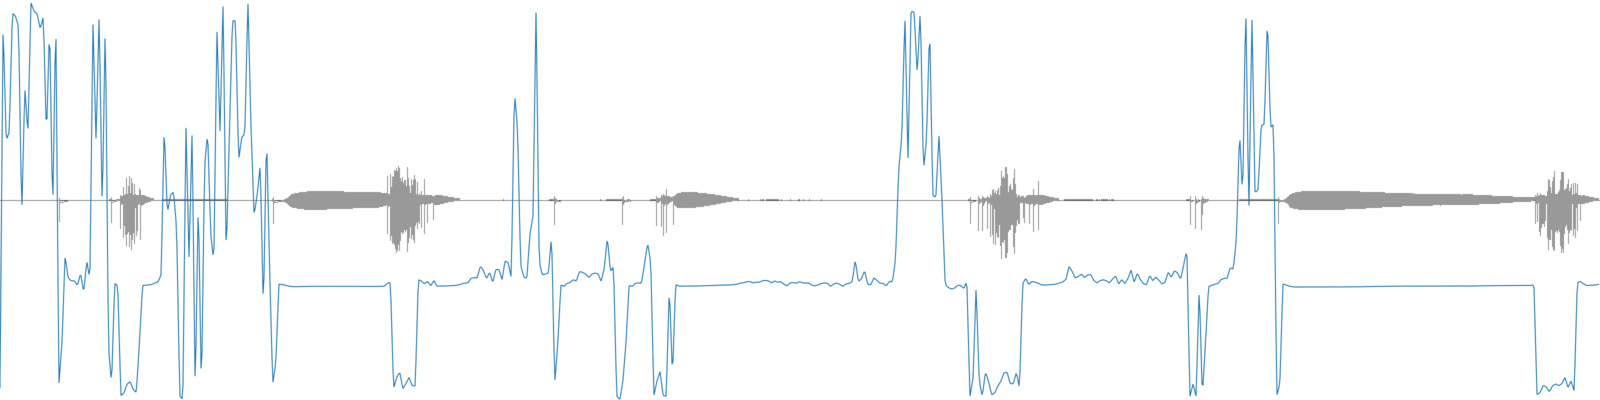
\includegraphics[width=0.9\textwidth]{./figures/pitch-analysis.jpg}
\caption{Pitch analysis of a buffer that has some pure tone and some scratchy timbres.}
\label{fig:pitch-analysis}
\end{figure}

Another useful outcome of this activity can be acknowledged when
discussing \href{https://learn.flucoma.org/learn/why-scale/}{Distance as
Similarity}. Most listeners will sing the correct pitch class but down a
few octaves. For these listeners, being 12 half steps lower (a distance
of 12) is closer than being 1 half step lower (a distance of one). This
is again a recognition that what humans might assume to be
\emph{similar} a machine might not (in this case using
\href{https://learn.flucoma.org/reference/chroma/}{Chroma} analysis may
help align human and machine listening).

\subsubsection{Statistics}

Many workflows in FluCoMa require the use of statical summaries of audio descriptor time series, real time audio analyses, or whole DataSets. It is important for
learners to develop a sense of what tools are available and why one
might reach for one statistical summary rather than another.

\href{https://learn.flucoma.org/reference/bufstats/}{BufStats} is
perhaps the most commonly used object in FluCoMa and therefore has a
somewhat involved reference page. Many of the statistics available might
be familiar to learners (mean, median, minimum, and maximum), while
others might be new (standard deviation, skewness, kurtosis,
derivatives, etc.). During the introductory tutorials, many moments arise that are useful for reflecting on the statistical analyses being used and how they affect the sonic results being heard. A few examples are
\href{https://youtu.be/sabA8p8Y-Xs?t=1311}{reflecting on what it means
to have an average spectral centroid of a sound slice} and
\href{https://youtu.be/qom6x1u4_6A?t=1437}{using the maximum value of an
analysis rather than the mean}.

BufStats has many more features that are somewhat less explored and
probably not appropriate for learners just getting acquainted with
FluCoMa. There are few Learn Articles that cover these topics in
musicianly ways including
\href{https://learn.flucoma.org/learn/weighting-stats/}{Weighting Stats}
and \href{https://learn.flucoma.org/learn/outliers/}{Outliers}. It is
also important to convey to learners, as is stated on the
\href{https://learn.flucoma.org/reference/bufstats/}{BufStats} page,

\begin{quote}
\emph{While it can be difficult to discern how to use some of these
analyses practically (i.e., what does the kurtosis of the first
derivative of spectral centroid indicate musically?), these statistical
summaries can sometimes represent differences between analyses that
dimensionality reduction and machine learning algorithms can pick up on.
Including these statistical descriptions in training or analysis may
provide better distinction between data points.}
\end{quote}

\subsubsection{``Know Your Data''}

As with all data science and machine learning, understanding what data
represents, what it can tell you (and more importantly what it
\emph{can't}), and what transformations \emph{do} to data is essential.
It is continuously important for FluCoMa learners to reflect on their
data. There are a few visualization tools that are very important for
users to get comfortable with including the Waveform object
(\texttt{fluid.waveform\textasciitilde{}} in Max and
\texttt{FluidWaveform} in SuperCollider). While teaching, these tools
should be used whenever possible to help learners understand the data
processing that is happening and get them in the habit of visually
checking on their data regularly to build understanding of what their
data represents.

Many machine learning algorithms make various assumptions about data
(similar to how humans make assumptions about sound and machine
listening). One of these assumptions is that the dimensions in a DataSet
are identically distributed, often Gaussian distributed. It can be
important to know how one's data is distributed and it is possible to
check on using a histogram. Our
\href{https://learn.flucoma.org/learn/distribution/}{Distribution and
Histograms} page gives some examples of different kinds of
distributions, what they mean, and some example code to check on a
distribution using a histogram.

\subsubsection{Scalers \& Distance as Similarity}

Another important concept for learners to understand is how measures of
distance impact perceptions and assumptions about similarity. Once the
machine has ``listened'' and a statistical summary has been computed, a
next step is often to compare data points by computing the distance
between them (most of the FluCoMa tools use Euclidean Distance).
Computing distance very quickly makes questions about ranges and scaling
relevant, such as how a
\href{https://youtu.be/qom6x1u4_6A?t=1122}{mismatch of scale} may
overly weight the importance of dimensions that have larger ranges.

This is a great opportunity to
\href{https://learn.flucoma.org/learn/comparing-scalers/}{compare
scalers} available in FluCoMa. One way of clearly demonstrating that
different scalers will have different sonic results (and that those
sonic results are not always \emph{predictable}) is to choose a single
point in a DataSet (such as one sound slice), and find what the nearest
neighbor is with (1) no scaling, (2) Normalize, (3) Standardize, and
(4) RobustScale. (This is essentially what the sequence of images does in
the \href{https://learn.flucoma.org/learn/comparing-scalers/}{Comparing
Scalers} page.) Doing these comparisons in real time while hearing the sonic differences
can help concretize the importance for learnings.

It can often be important for learners to keep track of which dimensions
might be logarithmic or linear and know how those differences could
affect measures of distance. One concrete example we provide is on our
scaling page under the heading
\href{https://learn.flucoma.org/learn/why-scale/\#linear-vs-logarithmic-scales}{Linear
vs Logarithmic Scales} where we state:

\begin{quote}
\emph{For example, frequency analyses might be provided in hertz (which
is on a linear scale), however this doesn't reflect how humans actually
perceive pitch distance. For a more perceptually relevant scale it is
displayed logarithmically in pitch space (perhaps labeled as MIDI notes
or semitones). If measuring in hertz, the distance from the A4 down one
octave to A3 is 220 hertz, while the distance from A4 up one octave to
A5 is 440 hertz---twice as far even though we perceive them to both be
one octave! Measuring these distances in semitones however will reflect
they way we perceive them: both a distance of 12.}
\end{quote}

FluCoMa objects which analyze for frequency have an argument called \texttt{unit} which specifies if the frequency estimation should be returned in Hz or MIDI notes.

\subsubsection{Human vs. Machine Assumptions}

One more concrete example of how human and machine assumptions differ
comes from a learner who has having trouble getting
\href{https://learn.flucoma.org/reference/kmeans/}{KMeans} to cluster
data points in they way they thought it should. The learner wanted
KMeans to cluster
\href{https://discourse.flucoma.org/uploads/default/original/2X/2/25c1edfb63797e7fd4051872088e6610ce908981.jpeg}{points on a 
2D plot} according to the clusters that are easily visually identifiable
by a human. KMeans was clustering it much differently,
including leaving many clusters empty. This was solved by
\href{https://www.youtube.com/watch?v=LzoWRqZzhZ4}{demonstrating}
(including \href{https://www.youtube.com/watch?v=mFsuJXqNYFs}{with the
original data}) how the learner could seed KMeans as a ``human in the
loop'' approach to direct its processing with the information also
inferred by a human.

\subsection{De-Myth-ifying Machine Learning}\label{de-myth-ifying-machine-learning}

Sometimes we have questions from learners that sound something like, ``I
want X to do Y. How can FluCoMa do this?''. At this point, our
pedagogical step is to break down the goal into smaller and more
specific questions and tasks that we can start approaching together with
the learner. This process often reveals the assumptions that the learner
might be making about how audio analyses work, or what a machine will be
able to perceive, or how long an analysis or algorithm might take, and
all of the tradeoffs involved in making decisions about the process.
Sometimes the question transforms from ``How can FluCoMa do this?'' to
``Can FluCoMa do this?'' at which point perhaps there's a different tool
that we can point them to, or help them realize that their goal is too
lofty--that it stems from a belief that ``AI can do anything'' or
``throw it at a neural network and it'll figure it out''. Usually this
process enriches the learners ideas about what is possible with FluCoMa
(even if it's not necessarily what they hoped) and provides a lot of
possibilities for investigation.

Another de-myth-ification that has occured is when learners will assume
that the machine learning \emph{is} performing some magic. This is often
in the form of learners not \emph{validating} or testing the machine
learning model or the results of their algorithm. The first disclaimer
to make is that, as artists, we're interested in artistically compelling
experiences, so regardless of what the algorithm is or isn't doing, if
it sounds good, keep it. It is also important to test the systems that
we build and see if they are doing what we think they're doing. This is
important for a few reasons:

\begin{itemize}
\tightlist
\item
  Validation can reveal our assumptions and/or misunderstandings about
  \emph{how} things work, providing opportunities to deepen our
  knowledge and skills.
\item
  Validation can offer ways to improve our system to get even closer to our
  desired outcome.
\item
  Validation can reveal nuances in the system that might offer more paths of
  exploration and creativity.
\end{itemize}

Framing validation with these benefits in mind can help encourage
learners to put in the extra work that it takes.

\subsection{CCE Specific Objects}\label{cce-specific-objects}

Pedagogues should be aware that there are a few objects in FluCoMa that
are CCE specific in name and/or implementation because of CCE
differences. These objects diverge from FluCoMa's philosophy of
cross-environment parity in order to ensure workflows in the toolkit are
idiomatic and \emph{Fluid} for beginner and expert users. When teaching a room that has learners using multiple CCEs it is important to be highlighting the differences in the course of the lesson to ensure understanding. The main differences regard interfacing with Buffers.

\textbf{Writing control information into a buffer}

\begin{longtable}{ll}
\toprule
Max & fluid.list2buf \\
SuperCollider & FluidKrToBuf \\
Pure Data & (native) \\
\bottomrule
\end{longtable}

\textbf{Reading control information out of a buffer}

\begin{longtable}{ll}
\toprule
Max & fluid.buf2list \\
SuperCollider & FluidBufToKr \\
Pure Data & (native) \\
\bottomrule
\end{longtable}

\textbf{The FluCoMa Plotter object has similar functionality and syntax
across all three CCEs but divergent implementation}

\begin{longtable}{ll}
\toprule
Max & fluid.plotter \\
SuperCollider & FluidPlotter \\
Pure Data & fluid.plotter \\
\bottomrule
\end{longtable}

\textbf{The FluCoMa Waveform object has similar functionality and syntax
across all three CCEs but divergent implementation}

\begin{longtable}{ll}
\toprule
Max & fluid.waveform\textasciitilde{} \\
SuperCollider & FluidWaveform \\
Pure Data & fluid.waveform \\
\bottomrule
\end{longtable}

\section{Relevance to Contemporary
Society}\label{relevance-to-contemporary-society}

We believe that learning about data, data science, and machine learning
through FluCoMa can be used as a lens to consider how these tools
operate in contemporary society, in particular to uphold inequalities,
injustices, and hegemonies. By gaining fluency and understanding with
these algorithms, one can come to understand what these algorithms are
good for, what they are not good for, how they go wrong, and the
relationship between data, algorithms, and the humans that use them. The
skills and knowledge, both explicit and tacit, that working with FluCoMa
fosters can be used to reflect on many of the AI events and concerns
that are constantly appearing in the news. Pedagogues might draw on
these events to use as discussion topics where a classroom of learners
can collectively reflect on contemporary topics using the experience and
understand built through FluCoMa.

Below is a list of books (in no particular order) that provide many
examples of contemporary technologies negatively impacting marginalized
communities. Many additionally offer directions for how to approach and
use data science ethically. We recommend selecting a book or selected
readings from these books to augment learning. Each of these is written
for different audiences, so selecting which is best is at the
instructor/learner's discretion.

\begin{itemize}
\tightlist
\item
  \emph{Data Feminism} by Catherine D'Ignazio and Lauren F. Klein.
\item
  \emph{Weapons of Math Destruction} by Cathy O'Neil
\item
  \emph{Hello World} by Hannah Fry
\item
  \emph{Revolutionary Mathematics} by Justin Joque
\item
  \emph{Blockchain Chicken Farm: And Other Stories of Tech in China's
  Countryside} by Xiaowei Wang
\item
  \emph{The Alignment Problem} by Brian Christian
\end{itemize}

\bibliographystyle{plain}
\bibliography{bibliography}

\end{document}